\documentclass[12pt]{article}
\usepackage[ngerman]{babel}
\usepackage[utf8]{inputenc}
\usepackage{hyperref}
\usepackage{graphicx}
\usepackage{textcomp}
\usepackage[export]{adjustbox}
\usepackage[doublespacing]{setspace}

\title{Programmierprojekt 3}
\date{\copyright\today}

\parindent 0pt
\def\labelitemii{$\bullet$}
\raggedright

\begin{document}
	
	\newpage
	
	\section{Nutzerhandbuch}
	
	Dieses Nutzerhandbuch soll in die vorliegende Anwendung einweisen. \newline Die aktuellste Version befindet sich auf github unter \url{https://github.com/ProPra16/programmierpraktikum-abschlussprojekt-goldener-ring}.
	Die Anwendung soll beim Üben des Test Driven Development behilflich sein. Eine genauere Erklärung dieses Verfahrens ist dieser Text von Frank Westphal (\url{http://www.frankwestphal.de/TestgetriebeneEntwicklung.html}).
	\newpage
	\section{Grundlegende Bedienung}
	
	    \begin{figure} [htbp]
	    	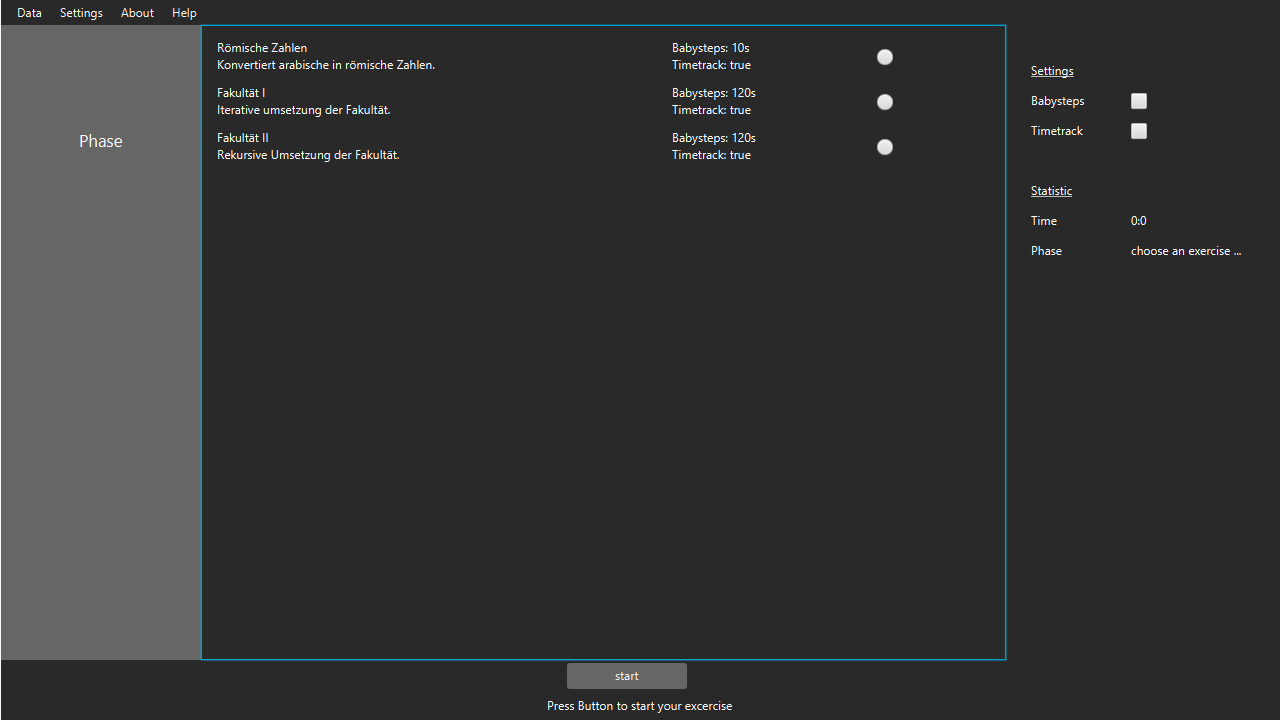
\includegraphics[width=1\textwidth]{figures/gui}
	    	\caption{GUI mit Beispielskatalog}
	    	\label{gui}
	    \end{figure}
	    	
		Die Oberfläche ist nach einem Borderpane aufgebaut. 
		Gesteuert wird die Anwendung größtenteils über die unteren Flächen. Dort sind Buttons zum Navigieren angebracht. \newline
		Über die obere Menüleiste ist es möglich zum Katalog zurückzukehren, wie auch einen Guide (englisch) zu öffnen.
		Es sind zwei verschiedene Designs für die Anwendung verfügbar, die ebenfalls über die Menüleiste gewechselt werden können. \newline
		Im Zentrum befindet sich zu Anfang der Katalog. Im Katalog sind die ausgelesenen Aufgaben mit Konfiguration aus der Katalog.xml aufgeschrieben. \newline Ob Babysteps oder Tracking eingeschaltet wird ist optional und kann über zwei Boxen an der rechten Seite eingestellt werden. Im Katalog selber wählt man eine Aufgabe über die Radioboxen an.
		Während der Aufgabe ist statt dem Katalog ein TextArea vorhanden, in dem der Code geschrieben werden soll.
		
		\begin{figure} [htbp]
			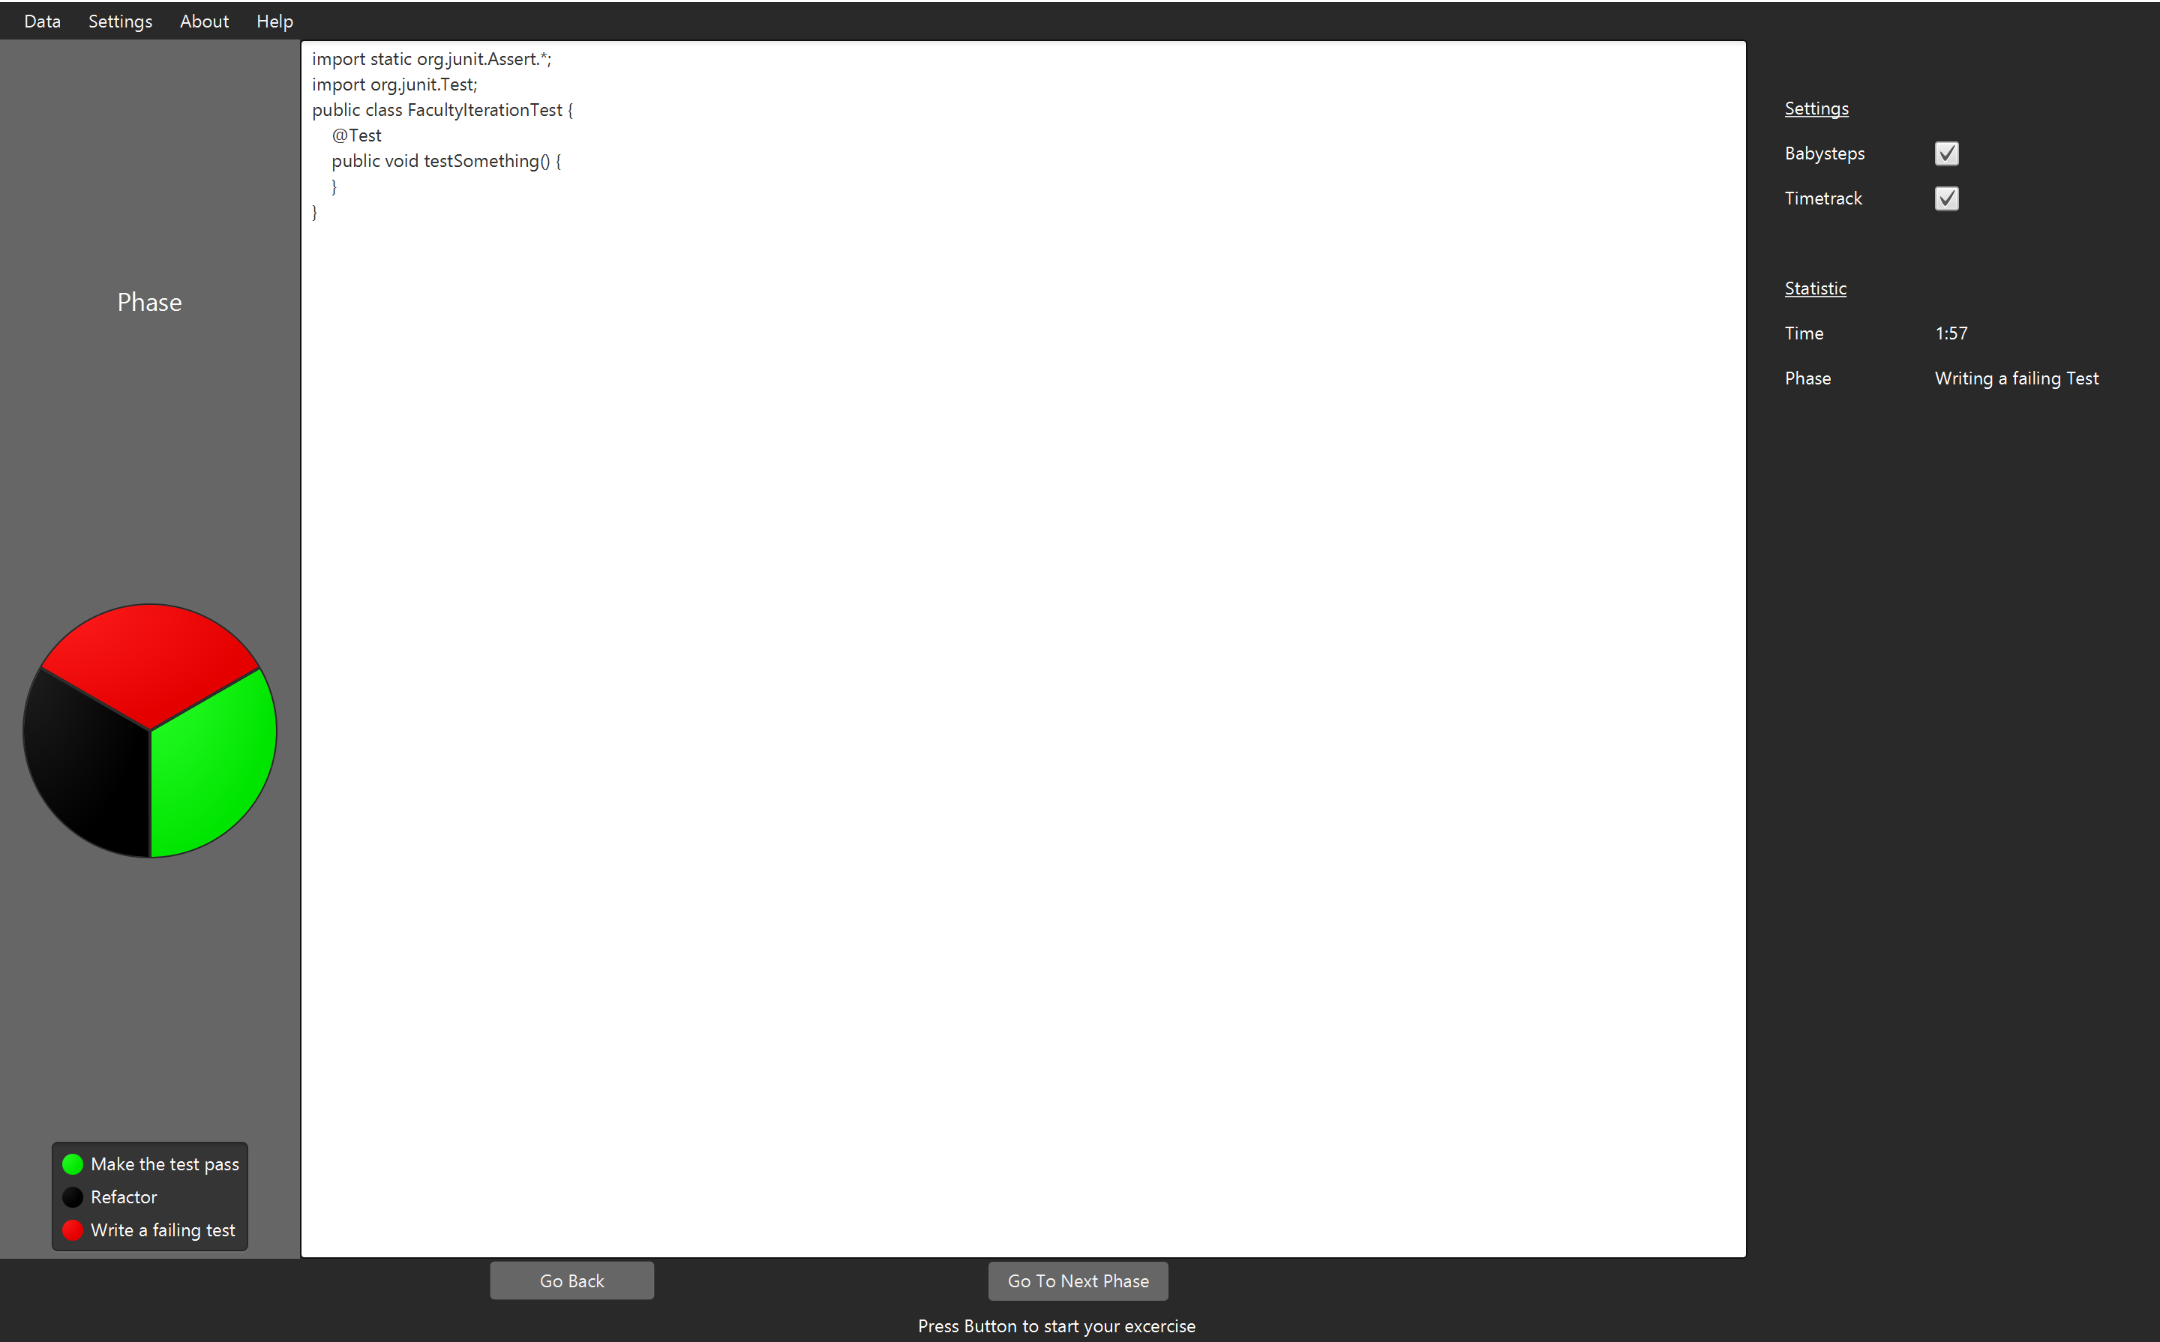
\includegraphics[width=1\textwidth]{figures/guiArea}
			\caption{GUI mit Beispielstest}
			\label{guiArea}
		\end{figure}
		
		An der rechten Seite befindet sich eine Beschreibung der aktuellen Phase, sowie einen Timer im Falle von aktivierten Babysteps. Auf der linken Seite ist eine graphische Repräsentation der Phase, mit der aktuellen nach oben ausgerichtet.
		Sollte Tracking eingeschaltet sein, gibt es am Ende ein Liniendiagramm.
\end{document}